\documentclass[12pt]{unlsilabsop}

\title{Master SOP}
\date{Juli 6, 2015}
\author{Frank Meier Aeschbacher}
\approved{Frank Meier Aeschbacher}
\sopid{000}
\sopversion{v0}
\sopabstract{This master document describes the operations at UNL for manufacturing and testing modules within the \emph{CMS Pixel Phase-I} upgrade project. It describes responsibilities, local organization and the documentation structure.}
\begin{document}

\maketitle

%-------------------------------------------------------
\section{Scope}
The high energy physics group at University of Nebraska-Lincoln hosts one of the two US manufacturing sites for sensor modules to be used in the upgraded CMS forward pixel detector. Most of the activities are carried out in the lab (room JH~174) and the cleanroom inside there (room JH~174C).

%-------------------------------------------------------
\section{Purpose}
This document and the herein listed subdocuments describe the procedures in place to manufacture modules to high standards and principles to assure their quality.

%-------------------------------------------------------
\section{Definitions}
The definitions defined here apply to all subdocuments as well.
\begin{description}
    \item[BBM] \emph{Bare bump-bonded module.} Consists of a silicon sensor and 16 ROC, attached through bump bonding.
    \item[HDI] \emph{High-Density Interconnect}. Flexible circuit board providing connection from the ROC to the data acquisition systems. Carries a TBM.
    \item[ROC] \emph{Read Out Chip.} Chips attached to the sensors using bump bonding. Every pixel of the sensor is attached to an individual amplifier/comparator circuit on the ROC, which orchestrates the readout of signals for all pixels covered by one ROC.
    \item[TBM] \emph{Token Bit Manager.} Chip to control the readout of ROC in a module and providing interfaces to the outer world. Normally part of an HDI.
\end{description}

%-------------------------------------------------------
\section{Responsibilities}
\begin{itemize}
    \item The \textbf{main responsible} is the \emph{principle investigator}.

    Currently: Aaron Dominguez
    \item The \textbf{responsible for operations} maintains the SOP documents current, organizes the proper training and makes sure all members of the team follow the SOP. Reports to the \emph{main responsible}.

    Currently: Frank Meier
    \item \textbf{Team members} are responsible to follow the instructions described in the SOP documents for which they are trained. They are not allowed to carry out any procedure without proper and documented training~(\texttt{SOP-000-Form-01}). Pre-production is considered training phase where procedures are allowed to be carried out without documented training. Team members report to the \emph{responsible for operations}.

    The list of current team members is maintained by the \emph{responsible for operations}.
\end{itemize}


%-------------------------------------------------------
\section{Document hierarchy}
The documents are organised in a hierarchical way, as outlined by Fig.~\ref{fig:SOPhierarchy}.
\begin{figure}[h]
    \begin{center}
        \includegraphics[width=16cm]{img/SOPhierarchy.pdf}
        \caption{Hierachy of SOP documents. The three-digit number identifies documents and the first digit assigns it to a class.}
        \label{fig:SOPhierarchy}
    \end{center}
\end{figure}
Documents are identified by a 3-digit number. The top-level document has the number 000. All the other documents carry numbers different from this. The first digit identifies the group the document belongs to, see Fig.~\ref{fig:SOPhierarchy}.

\subsection{Document managements: versioning, repository}
Any SOP document carries a revision number, consisting of the letter `v' followed by a number. `v0' identifies a draft document. Any document `v1' and above is effective as of the date printed. Document versions may be used as follows:
\begin{itemize}
    \item Always use latest document available. CMS DocDB~\cite{SOPdocDB} is the ultimate source, with links on the TWiki page~\cite{UNLtwiki} provided for convenience.
    \item Only final versions become uploaded to DocDB, drafts are available from the TWiki only.
    \item Until the end of the \emph{pre-production} phase, draft documents are allowed to be used if no other released version is available.
    \item In \emph{production} phase, draft documents are no longer accepted.
\end{itemize}
The \LaTeX{} sources including all image files are stored in a git repository~\cite{SOPgit}, which keeps track of changes to the documents.

\subsection{Referencing documents}
\begin{itemize}
    \item Cross-reference within SOP documents go as SOP~XXX, where XXX is the document number. This assumes a reference to the latest version of that document. References to specific version are to be avoided.
    \item Referencing from external documents should use the full title and SOP number.
\end{itemize}

\subsection{List of documents}
Table \ref{tbl:SOPlist} shows the planned documents. They do not need to be in place before this document becomes v1. A list of all current documents is to be maintained and made accessible to all people involved.

\begin{table*}[hH]
\begin{center}
\caption{List of SOP documents}
\label{tbl:SOPlist}

\bigskip

{\footnotesize
\begin{tabular}{lp{7cm}p{6cm}}
\toprule
No. & Title & Comment \\
\midrule
000 & Master SOP & This document \\
\midrule
%001 & Production cycle and quality control & General process description \\
%002 & General documentation procedures & \\
%003 & Training & \\
001 & Access control & \\
002 & Backup and recovery & \\
003 & Protective measures & Personal protection, clean room rules, environmental protection \\
004 & Storage of raw, intermediate and finished parts & \\
\midrule
101 & Delivery of HDI & \\
102 & Delivery of BBM & \\
103 & Gluing of HDI to BBM & \\
104 & Wirebonding of modules & \\
105 & Encapsulation of wirebonds & \\
106 & Shipping of modules & \\
107 & Reworking of modules & \\
\midrule
201 & Visual inspection of HDI & \\
202 & Visual inspection of BBM & \\
203 & IV test of BBM & \\
204 & \emph{withdrawn} & \\ %204 & Electrical acceptance test of HDI & \\
205 & Visual inspection of final module & \\
206 & Electrical acceptance test of final module & \\
207 & Pull testing of wirebonds & \\
208 & \emph{withdrawn} & \\ %208 & Electrical acceptance test of BBM & \\
209 & Destructive wirebond acceptance test of HDI & Only for type-testing of new types or batches upon request \\
\midrule
301 & Cleanroom & \\
302 & Gantry & Covers glueing and encapsulation \\
303 & Wirebonder and pull tester & \\
304 & Probe station & \\
305 & Vacuum supply & \\
306 & Dry air supply & \\
307 & Cold box & \\
308 & HV power supply & \\
309 & Storage cabinets & \\
\bottomrule
\end{tabular}
}
\end{center}
\end{table*}


%-------------------------------------------------------
\section{Production life-cycle and critical control points}

The standard workflow is shown in Fig.~\ref{fig:WorkflowProduction}. Any normal module fulfilling all quality criteria will follow the standard path. Module quality is tested along the production path. Every such test defines a \emph{critical control point}. Modules failing the quality criteria will be judged for reworking or will be classified as bad.

Acceptance criteria and specifications are managed outside of UNL scope and are available at~\cite{FPixSpec}.

\begin{figure}[h]
    \begin{center}
        
\includegraphics[width=12.7cm]{img/WorkflowProduction.pdf}
        \caption{Standard workflow for production of modules at UNL. Solid paths show the steps all modules will undertake. Dashed paths are optional steps, based on needs (reworking if quality criteria not matched) or additional tests (according to testing schemes). Critical control points are shown as solid ellipses. Numbers refer to SOP documents.}
        \label{fig:WorkflowProduction}
    \end{center}
\end{figure}

%-------------------------------------------------------
\section{Documentation of workflow, test results and maintenance operations}
Any action following procedures covered by this set of SOP need to be documented as follows:
\begin{itemize}
    \item All activities need to be documented.
    \item Any activity that produces results or processes parts (raw, intermediate or finished) requires an update in the Purdue database~\cite{PurdueDB}. Instructions for this are included in the respective SOP.
    \item Additional documentation beyond what can be stored in the Purdue database or not covered by the workflow in there  (e.g.~maintenance activities) have to be documented on the elog~\cite{UNLelog}.
\end{itemize}

\subsection{Identification of parts and batches}
\begin{itemize}
    \item \textbf{BBM} are identified using the naming convention~\cite{BBMnaming}, which handles several cases. We have only the case of ``bump-bonded $2\times8$ modules''. The id is grouped as follows:
        \begin{itemize}
        \item \texttt{BL} to designate ``bump-bonded $2\times8$ modules''.
        \item \texttt{YY} to designate the position on the wafer, where \texttt{YY} is a two-letter code, see Fig.~\ref{fig:BBMwaferpos}.
        \item \texttt{ZZZ} to match to wafer numbers, where \texttt{ZZZ} are numbers. Preproduction sensors have the first digit always set to 9, followed by two numbers matching the wafer numbers. Production sensors use numbers in the range 001 to 200.
        \end{itemize}
    The components of the id are concatenated with underscores '\texttt{BL\_YY\_ZZZ}'.
    Example: \texttt{BL\_FL\_901} is a ``bump-bonded $2\times8$ module'' made from a sensor in the far-left position on the wafer and comes from pre-production wafer 1.

    The bump-bond manufacturer uses a different scheme which needs translation as follows:
        \begin{itemize}
        \item Preproduction modules come with a wafer number \texttt{AZZ}, which translates directly to \texttt{9ZZ}.
        \item Production modules may come with the number that can be directly used as our \texttt{ZZZ} (with leading zeroes).
        \item The position on the wafer is delivered as a number in the range 1 to 8. Use the mapping shown in Fig.~\ref{fig:BBMwaferpos} to translate those single-digit numbers into the two-character alphanumeric code.
        \end{itemize}

    \item \textbf{HDI} are identified by four numbers that are assembled to one string, separated by dashes~\cite{HDInaming}:
        \begin{itemize}
        \item Work order (\texttt{AAABB} where \texttt{AAA} are alphanumeric digits, \texttt{BB} are numeric digits)
        \item Date code (\texttt{WWYY} where \texttt{WW} is the week of the year and \texttt{YY} is the year)
        \item Panel and position number (\texttt{N-MM} where \texttt{N} is the panel number processed and \texttt{MM} is the position of the HDI on the panel)
        \end{itemize}
    This makes up the following unique id for an HDI: \texttt{AAABB-WWYY-N-MM}, for example:~\texttt{YHC69-1015-3-11}.

    Other information on an HDI can be safely disregarded. An example for a RevD (RevC) HDI is given in Fig.~\ref{fig:HDI_SN_RevD} (Fig.~\ref{fig:HDI_SN_RevC}).

    \item A \textbf{batch} at UNL is identified using a six-digit number of the format \texttt{Nxxxyy} where
        \begin{itemize}
        \item \texttt{N} identifies a batch number, N standing for Nebraska
        \item \texttt{xxx} is a three-digit number with leading zeroes identifying the group of modules within the batch, \texttt{001} referring to the first batch etc.
        \item \texttt{yy} is a two-digit number with leading zero identifying the individual modules inside a batch
        \end{itemize}
    Example: \texttt{N00403} is module \texttt{03} of batch \texttt{004}

    The list of batch numbers is maintained in a spreadsheet~\cite{UNLlist}.

    \item \textbf{Assembled modules} use an identification derived from the HDI~\cite{HDInaming}. The number is assigned by the Purdue database and consists of
        \begin{itemize}
        \item \texttt{X} identifies a preproduction module with \texttt{P} and a production module with \texttt{M}.
        \item \texttt{Y} is a one-letter code to enumerate the prefixed batch information on an HDI (\texttt{AAABB-WWYY} as explained above). The list of such codes is maintained within the Purdue database. The first batch will receive the letter \texttt{A} and so on.
        \item \texttt{N-MM} is the panel and position number as used in the identification of HDI.
        \end{itemize}
    Example: \texttt{P-A-3-11}. Assuming \texttt{YHC69-1015} translates to the batch id~\texttt{A} this would be the module made out of the example HDI used above.
\end{itemize}

\begin{figure}[hH]
    \begin{center}
        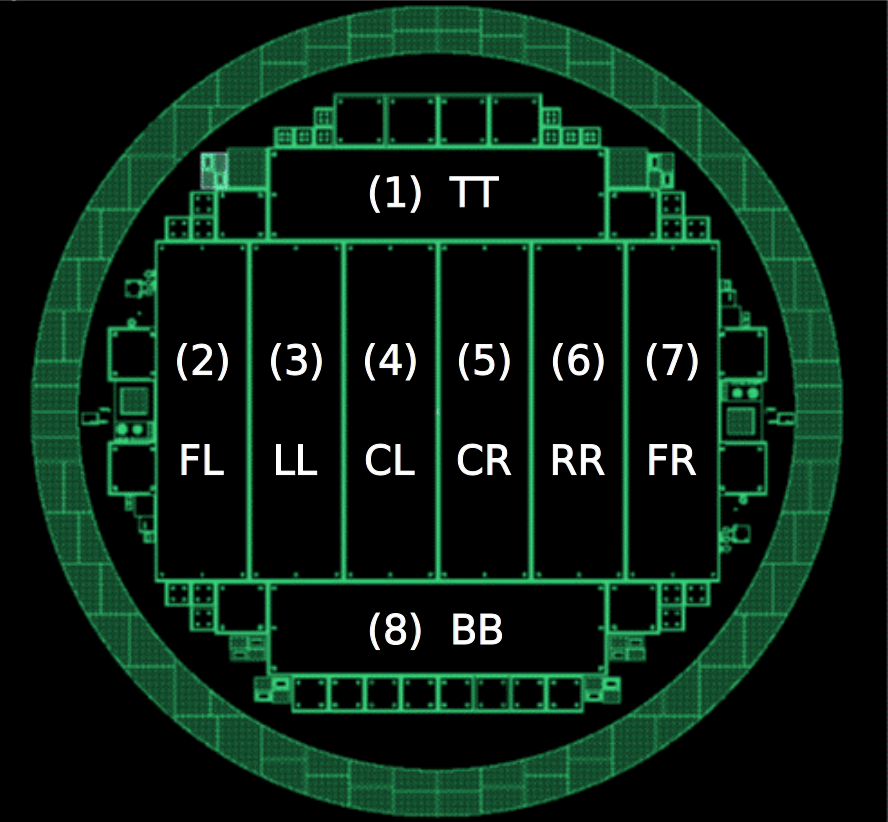
\includegraphics[width=7cm]{img/SensorsWaferposPurdueconvention.png}
        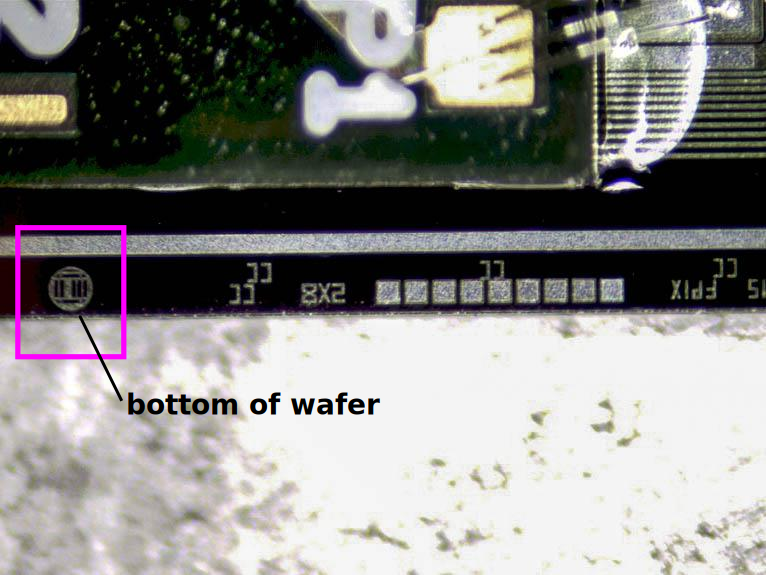
\includegraphics[width=7cm]{img/SensorIDonSensor.jpg}
        \caption{\textbf{Sensor wafer positions.} Left: Wafer sketch as seen from p-side. Numbers in parenthesis are the numbers used by the bump-bonding manufacturer, two-letter codes follow the Purdue-convention~\cite{BBMnaming}. Actual wafer layouts may differ, image shown as example. Right: Wafer icon as it can be viewed on a sensor edge. The orientation matches the left sketch. In this example, the sensor comed from a CL position.}
        \label{fig:BBMwaferpos}
    \end{center}
\end{figure}

\begin{figure}[hH]
    \begin{center}
        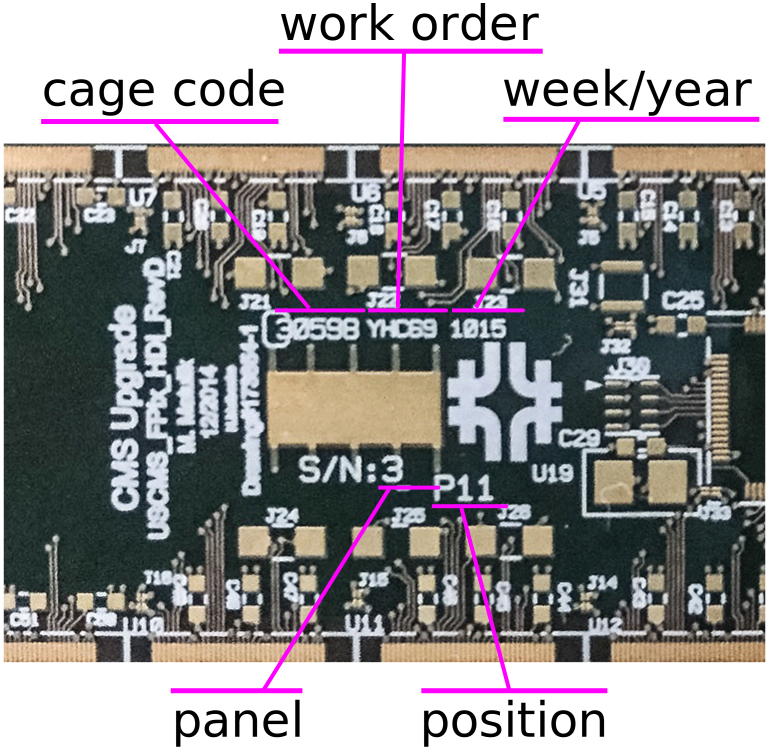
\includegraphics[width=7cm]{img/HDIRevD_id.png}
        \caption{\textbf{Example to identify an HDI (RevD):} ID of this HDI would be \texttt{YHC69-1015-3-11}, meaning work order \texttt{YHC69}, manufactured in week 10 of year 2015, third panel processed in this batch, and this is HDI from position 11 of that panel. All other information can be safely disregarded, especially the number \texttt{30598} (which is an internal cage code used by the manufacturer).}
        \label{fig:HDI_SN_RevD}
    \end{center}
\end{figure}

\begin{figure}[hH]
    \begin{center}
        \includegraphics[width=5cm]{img/HDI_SN.jpg}
        \caption{\textbf{Example to identify an HDI (RevC):} ID of this HDI would be \texttt{YGU25-1814-1-25}, meaning work order \texttt{YGU25}, manufactured in week 18 of year 2014, first panel processed in this batch, and this is HDI from position 25 of that panel. All other information can be safely disregarded, especially the number \texttt{30598} (which is an internal cage code used by the manufacturer).}
        \label{fig:HDI_SN_RevC}
    \end{center}
\end{figure}

%-------------------------------------------------------
\section{Training}
\begin{itemize}
\item Training normally consists of instruction by the responsible supervisor or another trained staff member.
\item Documentation: Training status needs to be documented using form \texttt{SOP-000-Form-01} and kept on records with the responsible.
\end{itemize}

%-------------------------------------------------------
\section{Deviations from SOP}
Two cases need to be distinguished:
\begin{description}
    \item[Planned deviations] This can happen e.g.~upon special request to study certain changes to the procedures or due to specific circumstances (supplier issues, material changes etc.). Before starting the procedure, a written document needs to be signed off and a copy needs to be kept on record in the elog. In this document, the following topics need to be addressed: foreseen deviation, reason for doing so, risk assessment. The responsible for operations or the main responsible decide if they can take over the responsibilities, otherwise sign-off needs to happen by project management.
    \item[Unforeseen deviations] This can happen when a special condition required a deviation. Such cases need to be documented within ample time by the person observing the deviation and require sign-off by a site responsible. The latter decide if special action is required and decide if project management needs to be informed about the deviation. Documentation takes place as comments in the Purdue database plus a note in the elog.
\end{description}

%-------------------------------------------------------
\begin{thebibliography}{aaaaaaaa}
    \bibitem{SOPdocDB} \url{https://cms-docdb.cern.ch/cgi-bin/DocDB/ShowDocument?docid=12623}
    \bibitem{UNLtwiki} \url{https://twiki.cern.ch/twiki/bin/view/CMS/UNLPixelPhaseI}
    \bibitem{SOPgit} \url{https://github.com/frmeier/sop}
    \bibitem{FPixSpec} The specification and acceptance criteria document doesn't exist as of time of writing this document.
    \bibitem{PurdueDB} \url{http://www.physics.purdue.edu/cmsfpix/Submission_p/index.php}
    \bibitem{UNLelog} \url{http://t3-sl5.unl.edu:8175/SiLab_Logbook/}
    \bibitem{BBMnaming} \url{https://cms-docdb.cern.ch/cgi-bin/DocDB/ShowDocument?docid=12227}
    \bibitem{HDInaming} Reference to be added as soon as known, information based on internally circulated draft.
    \bibitem{UNLlist} \url{http://cern.ch/go/H897}
\end{thebibliography}
URL listed here may change over time and do not necessarily trigger a new version of this document. In case a link is broken, consult the TWiki page, which may have a newer link.

\end{document}

